\section{Simulation}

\pgfplotstableread[row sep=\\,col sep=&]{
    cristal                                                  & Serie 1 & Serie 2 & error_1   & error_2\\
    Cristal cylindrique                                      & 1430.18 & 955.978 & 563.49092 & 372.5446266 \\
    Cristal cuboide (\qtyproduct{20x20x76.96}{\milli\metre}) & 2221.99 & 963.492 & 709.925805 & 255.1326816 \\
    Cristal cuboide (\qtyproduct{20x20x75}{\milli\metre})    & 2092.62 & 1502.45 & 613.55 & 399.65 \\
}\datatable
\begin{figure}[h!t]
    \centering
    \begin{subfigure}[t]{0.49\textwidth}
        \centering
        \begin{tikzpicture}
            \begin{axis}[
                    ybar,
                    enlarge y limits={value=0.15, upper},
                    width=1\textwidth,
                    legend style={at={(0.99,0.99)},
                            anchor=north east,legend columns=-1},
                    ylabel={Comptage (\unit{cps})},
                    ymin=0,
                    symbolic x coords={Cristal cylindrique,Cristal cuboide (\qtyproduct{20x20x76.96}{\milli\metre}),Cristal cuboide (\qtyproduct{20x20x75}{\milli\metre})},
                    xtick=data,
                    xticklabel style={text width=0.33\linewidth,anchor=north},
                ]
                \addplot+[error bars/.cd, y dir=both, y explicit] table[x=cristal,y=Serie 1, y error=error_1] {\datatable};
                \addplot+[error bars/.cd, y dir=both, y explicit] table[x=cristal,y=Serie 2, y error=error_2] {\datatable};
                \legend{Serie 1,Serie 2}
            \end{axis}
        \end{tikzpicture}
        \caption{Comparaison des comptages entre les cristaux cylindrique et cuboïdes}
        \label{fig:graph_simu_cristal}
    \end{subfigure}
    \begin{subfigure}[t]{0.49\textwidth}
        \centering
        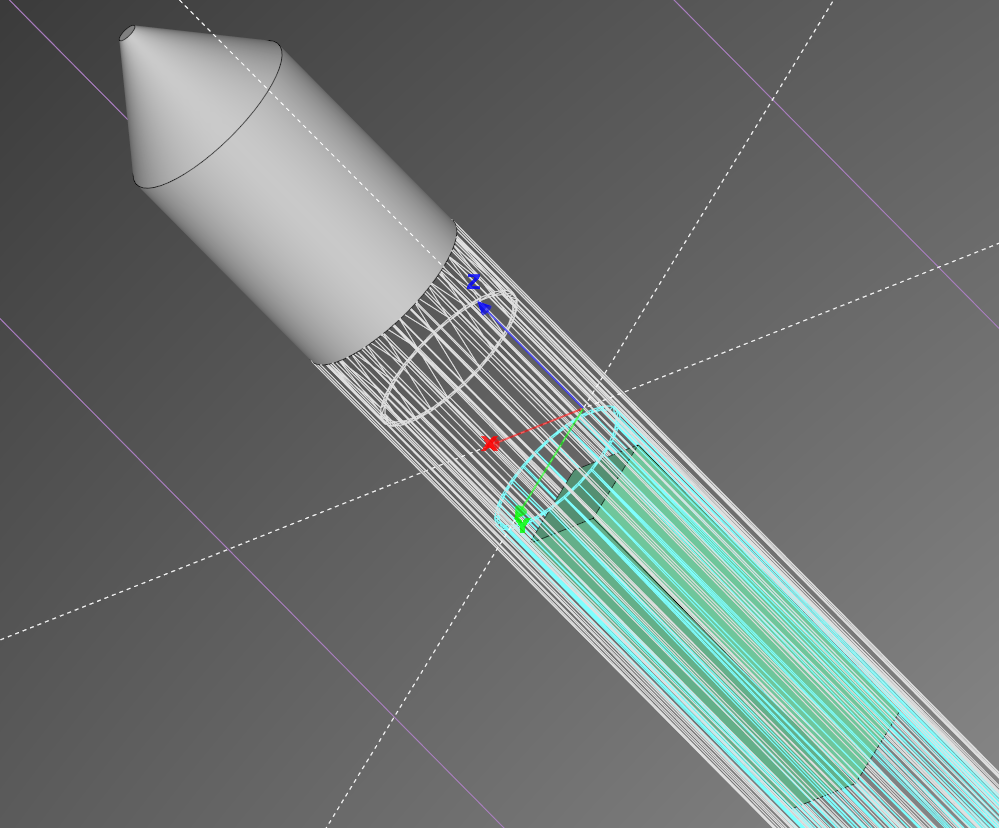
\includegraphics[width=0.7\textwidth]{photo/sonde_carre_simu.PNG}

        \caption{Capture d'écran de la simulation d'un cristal cuboïde}

    \end{subfigure}
    \caption{Simulation de détection de rayonnement gamma}
\end{figure}

Une différence entre les tubes photomultiplicateur et les SiPM est que les tubes photomultiplicateur ont une zone de détection en forme de rond alors que les SiPM ne peuvent qu’être produits en carré et donc limite les formes des zones de détection. Cela implique donc un changement de forme de cristal. Pour nous assurer que les anciens cristaux et les nouveaux se comportent de la même manière, nous allons faire une simulation. Les cristaux NaI à utiliser actuellement sont des cylindres de 28~mm de diamètre et 50~mm de hauteur. Pour que les nouveaux cristaux cuboïdes rentrent dans le boitier, ils doivent avoir une longueur et une largeur de 20~mm et pour que le volume, et donc normalement le nombre de détections, reste le même, ils doivent avoir une hauteur de 76,96~mm. Nous testerons également un cristal avec une hauteur de 75~mm pour voir si la petite différence de volume a un impact sur les résultats.

Un autre stagiaire a travaillé sur des sujets de simulation et a donc pu faire ces simulations pour moi. Malheureusement, il n'avait pas encore eu ses accès au serveur de calcul d'Orano et donc a dû les faire tourner à une plus basse résolution sur son ordinateur, ce qui explique les incertitudes important sur la figure \ref{fig:graph_simu_cristal}. %todo fix cref
